\documentclass[oneside,reqno]{amsart}
\setlength{\textwidth}{\paperwidth}\addtolength{\textwidth}{-2in}\calclayout
\usepackage{amsmath,amsthm}
\usepackage{dsfont} 
\usepackage{tikz}
\usepackage{enumitem}

\DeclareMathOperator{\E}{\mathrm{E}}
\DeclareMathOperator{\var}{\mathrm{var}}
\DeclareMathOperator{\cov}{\mathrm{cov}}
\newcommand{\eps}{\varepsilon}
\newcommand{\Ncal}{\mathcal{N}}
\newcommand{\Ucal}{\mathcal{U}}
\newcommand{\Z}{\mathds{Z}}
\newcommand{\R}{\mathds{R}}
\newcommand{\N}{\mathds{N}}
\theoremstyle{definition}
\newtheorem{prob}{Problem}
\renewcommand*{\proofname}{Solution}
\setlist[enumerate]{label={(\roman*)}}

\title{STAT 433: Homework 4}
\author{Daniel Pfeffer}
\date{\today}
%------------------------------------------------------------------------------
\begin{document}
\maketitle


\begin{prob}
Consider the following directed webgraph, where each edge has a direction. The web surfer can only jump along the assigned direction of the edge -- jumping in the reverse direction is prohibited. Let $X_n$ be a simple random walk of a web surfer on this graph. More precisely, if the surfer is at site $i$, then it will randomly pick one of the outgoing edges and jump to its neighborhood along this edge. For example, if the surfer is at site $c$, then it will choose one of the three outgoing edges, and jump to site $a$, $b$ or $d$ with probability $1/3$.
\begin{center}
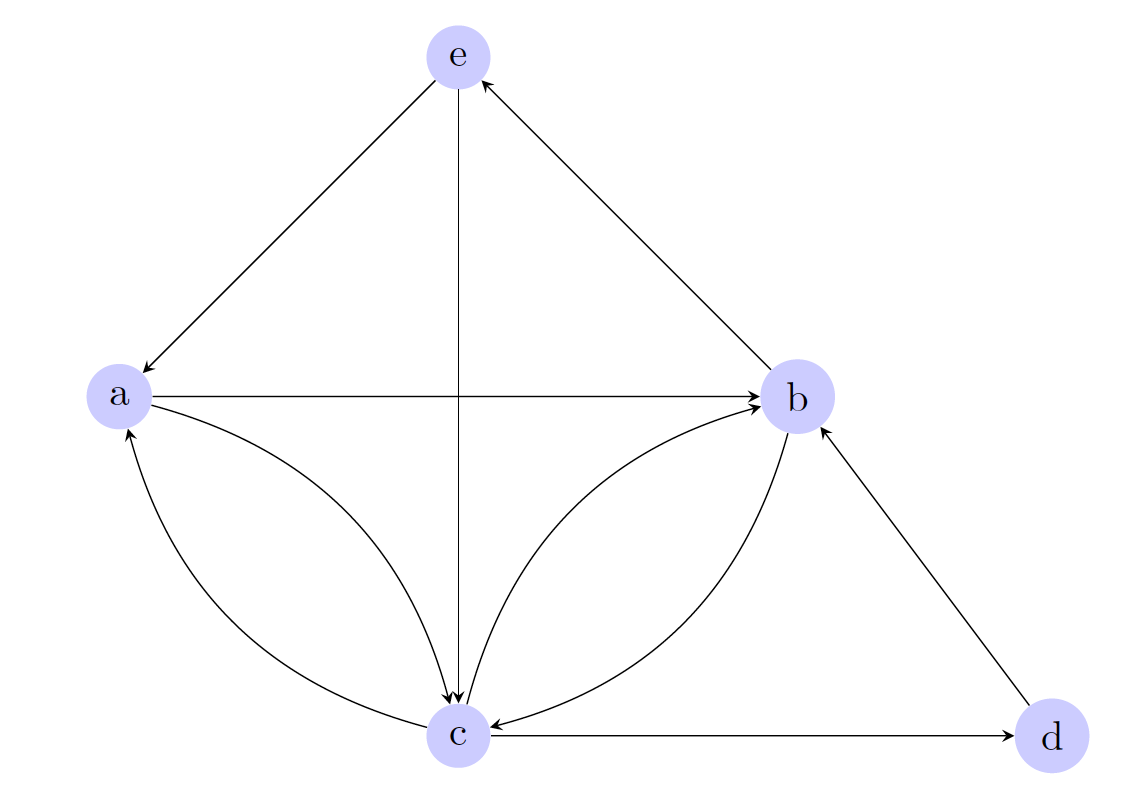
\includegraphics[scale=0.5]{webgraph}
\end{center}
\end{prob}

\begin{enumerate}
\item
Write down the transition matrix of this Markov chain.
\begin{proof}
Let $G=(V,E)$ be the webgraph where the vertex set $V=\{a,b,c,d,e\}$ and the edge set $E =\{(a,b), (a,c), (b,c), (b,e), (c,a), (c,b), (c,d), (d,b), (e,a), (e,c)\}$. Here the edge set contains ordered pairs where for any two vertices $i,j \in G$, $(i,j)$ represents the edge from $i$ to $j$.  Then the transition matrix is 
\[
	p(i,j) = P(X_{n+1} = i \mid X_n = j) 
	= \begin{cases}
		1/2 & \text{if } i=a, j=b,c \\
		1/2 & \text{if } i=b, j=c,e \\
		1/3 & \text{if } i=c, j=a, b, d \\
		1 & \text{if } i=d, j=b \\
		1/2 & \text{if } i=e, j=a,c. 
	\end{cases}
\]
Each entry is nonnegative and each row sums to one. Hence, $P$ is a transition matrix.
\end{proof}

\item
Show that the Markov chain is irreducible.

\begin{proof}
To demonstrate that this chain is irreducible, we show by inspection that for any initial state $i$ it is there is a nonzero probability of reaching any other state, i.e., the vertex set (state space) $V$ is a single communicating class. For the chain started at $a$, 
\begin{align*}
	p(a,b) &= 1/2>0 \\
	p(a,c) &= 1/2>0 \\
	p(a,d) &= p(a,b)p(b,c)p(c,d) = 1/2 \cdot 1/2 \cdot 1/3 \cdot >0 \\
	 p(a,e) &=p(a,b)p(b,e) = 1/2 \cdot 1/2>0. 
\end{align*}
For the chain started at $b$, 
\begin{align*}
	p(b,a) &= p(b,c)p(c,a) = 1/2 \cdot 1/3 >0 \\
	p(b,c) &= 1/2 > 0 \\
	p(b,d) &= p(b,c)p(c,d) = 1/2 \cdot 1/3 >0 \\
	p(b,e) &= 1/2 > 0.
\end{align*} 
For the chain started in $c$,
\begin{align*}
	p(c,a) &= 1/3>0 \\
	p(c,b) &= p(c,a)p(a,b) = 1/2 \cdot 1/2 > 0 \\
	p(c,d) &= 1/3>0 \\
	p(c,e) &= p(a,c)p(a,b)p(b,e) =1/3 \cdot 1/2 \cdot 1/2 >0. 
\end{align*}
For the chain started in $d$, 
\[
	p(d,a) =p(d,b) p(b,e) p(e,a) = 1 \cdot 1/2 \cdot 1/2 > 0,
\]
and as just shown, every state is accessible from $b$ and hence every state is accessible from $d$. For the chain started in $e$, 
\[
	p(e,a) = 1/2>0,
\] 
and again since every state is accessible from state $a$, every state is also accessible from $d$. Since every state leads to every other states, all states communicate with each other, and so the chain is irreducible.
\end{proof}

\item
Find the stationary distribution $\pi$. 

\begin{proof}
More explicitly, the transition matrix is
\[
	P=\begin{pmatrix}
		0 & 1/2 & 1/2 & 0 & 0 \\
		0 & 0 & 1/2 & 0 & 1/2 \\
		1/3 & 1/3 & 0 & 1/3  & 0 \\
		0 & 1 & 0 & 0 & 0  \\
		1/2 & 0 & 1/2 & 0 & 0	
	\end{pmatrix}
\]
It has stationary distribution $\pi = (6/35, 2/7, 3/10, 1/10, 1/7)$.
\end{proof}

\item
Determine the PageRank for the sites and explain the reasons.

\begin{proof}
The PageRank is $c$, $b$, $a$, $e$, and then $d$, which corresponds to the frequencies from the limiting distribution in (iii). 
\end{proof}

\end{enumerate}

\end{document}
